\documentclass[12pt,a4paper]{article}

\usepackage{hyperref}
\usepackage{graphicx}
\usepackage{float}
\usepackage{hhline}
\usepackage{datetime}
\usepackage{times}
\usepackage[margin=1cm]{geometry}
\hypersetup{hidelinks}

\title{
    A report about Creating a LoRa Satellite Ground Station  \\
    %  add a link to the station page for proof https://tinygs.com/station/MakerereUniversityRFOne@7818997512
    \vspace{0.5cm}
    \small{
        \href{https://tinygs.com/station/MakerereUniversityRFOne@7818997512}{https://tinygs.com/station/MakerereUniversityRFOne@7818997512}
    } \\
    \vspace{0.5cm}
    \large Using the TinyGS Project \\
}
\author{Group 2}
\date{\today}

\begin{document}

\maketitle

\begin{center}
    \renewcommand{\arraystretch}{1.5} 
    \begin{tabular}{|c|l|l|}
        \hline
        \textbf{No.} & \textbf{Name} & \textbf{Reg. No.} \\
        \hline
        1 & Shawal Mbalire & 21/U/0851 \\
        \hline
        2 & Abdulhakim B. Lukwago & 21/U/0627 \\
        \hline
        3 & Ssendagire Gilbert & 17/U/1124 \\
        \hline
        4 & Besigye Mukama & 21/U/10507/PS \\
        \hline
        5 & Olupot Emmanuel & 20/U/16032 \\
        \hline
        6 & Aradi Alamin Abdallah & 18/X/40426/PS \\
        \hline
        7&Onyango Hilary &21/U/0842 \\
        \hline
        8 & Ochengel Sulaiman & 20/U/2540/PS \\
        \hline
    \end{tabular}
\end{center}



\section{Introduction}
The TinyGS project \cite{tinygs} forms the basis of this project. TinyGS is an open network of Ground Stations distributed around the world to receive and operate LoRa satellites, weather probes, and other flying objects, using cost-effective and versatile modules. With an active Telegram community and GitHub resources, it is possible to build a LoRa-based ground station. This report documents the process of setting up a ground station.

This report is structured as follows:
\begin{itemize}
    \item Installation
    \item Configuration
    \item Antenna Building
    \item Data Analysis
\end{itemize}

\section{Installation}
To install the TinyGS firmware, a supported device is required. A list of supported devices is available on the TinyGS GitHub page. For this setup, a LILYGO T3 v1.6 was selected as it is one of the supported devices, simplifying the process.

The device was connected to a computer, and the installer at \href{http://installer.tinygs.com}{TinyGS Installer} was accessed. This provides an online web installer for firmware installation. The installer supports Chromium-based browsers, so one should ensure that a compatible browser is used. The installation was completed by following the on-screen instructions.

\section{Configuration}
Following installation, the LILYGO device rebooted and created a WiFi network for configuration. Connection to this network, named ``My TinyGS,'' was established, and the configuration page was accessed via the IP address \texttt{192.168.4.1}.

The configuration steps included:
\begin{enumerate}
    \item Assigning a name to the station.
    \item Creating a password for accessing the admin dashboard.
    \item Determining latitude and longitude using an online service such as \href{http://latlong.net}{latlong.net}, and entering the values up to three decimal places.
    \item Obtaining MQTT credentials:
    \begin{itemize}
        \item Joining the Telegram group at \href{https://tinygs.com}{TinyGS}.
        \item Sending a private message to \texttt{@tinygs\_personal\_bot} with the command \texttt{/mqtt}.
        \item Entering the provided credentials, noting that the username might begin with a \texttt{-} character.
    \end{itemize}
    \item Selecting the appropriate board type under Board Configuration. For boards with screens, this enables display functionality. The selected board type was the 433MHz LILYGO T3\_V1.6.1.
    \item Applying the changes and optionally restarting the station, which causes the LILYGO to reboot and disconnect from WiFi.
\end{enumerate}

The LILYGO device then attempted to connect to the specified WiFi network and the TinyGS MQTT server. Upon successful connection, the station became viewable on the TinyGS website.

Two dashboards were accessible:
\begin{itemize}
    \item A local dashboard was available on the same WiFi network as the LILYGO, accessible via an IP address displayed on the device's screen (e.g., \texttt{192.168.226.28}). This allowed local monitoring and configuration editing.
    \item The TinyGS web dashboard was accessed by sending \texttt{/weblogin} to \texttt{@tinygs\_personal\_bot}, which provided a login URL for managing the station online.
\end{itemize}

From the web dashboard, information such as the antenna type and operating range was updated. A quarter-wave grounded antenna with an operating range of approximately 433 MHz was used. Additionally, a brief description of the station was added for other TinyGS users.

\section{Antenna Design}
Once the station was connected to TinyGS and the MQTT server, receiving packets from satellites required an efficient antenna design and an unobstructed sky view.

The TinyGS configuration site suggests various antenna designs, one of which is the \href{http://www.n1gy.com/simple-ground-plane-antennas.html}{quarter-wave grounded antenna design}. This design was implemented and demonstrated acceptable performance during daylight hours. The antenna was resoldered to avoid shortages between the ground and the antenna. The new solder job is shown in the image below.
\begin{figure}[H]
    \centering
    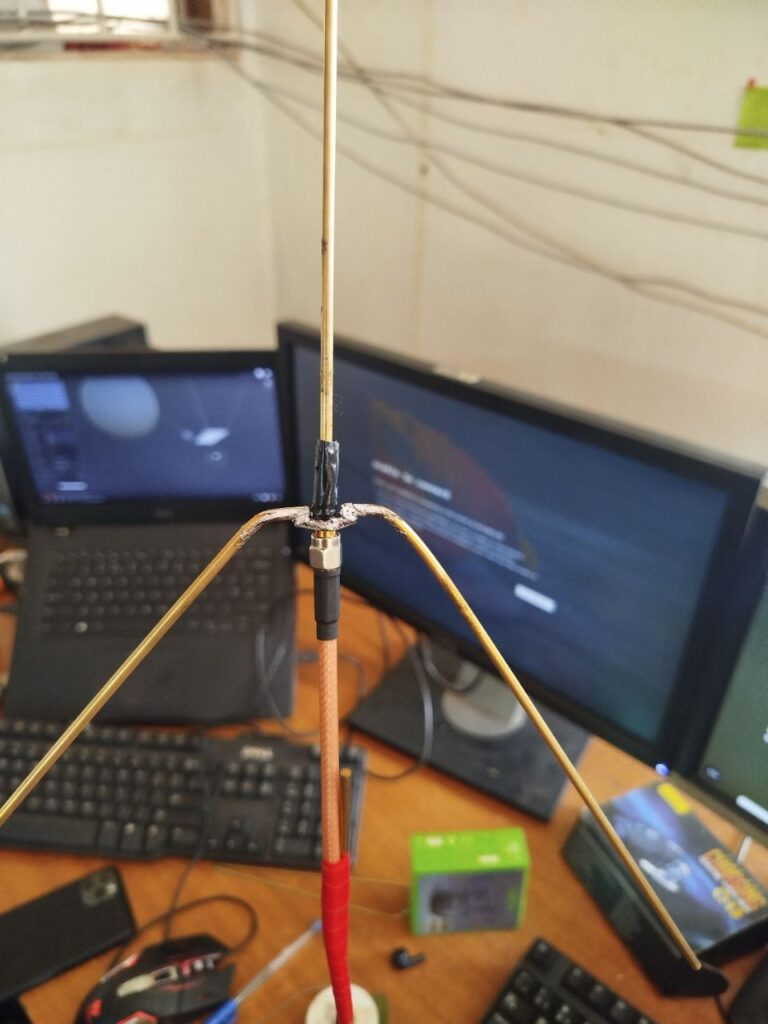
\includegraphics[height=0.5\textwidth]{../images/antennaeRedesign.jpg}
    \caption{Antenna solder job}
    \label{fig:antenna_solder_job}
\end{figure}

However, packet reception varied significantly depending on satellite coverage over Uganda.

\section{Data Analysis}
To evaluate the performance of the ground station, packet transmission data was collected over multiple days. 

% analysed columns = ['satelite',
%  'timestamp',
%  'Mode',
%  '📻 Power',
%  '📏 Distance',
%  '📐 Elevation',
%  '📶 RSSI',
%  'SNR',
%  'Predicted Doppler',
%  'Frequency Error',
%  'CRC Error',
%  'Received by']
The received data was picked from the website by webscrapping and majorly included the following columns:
\begin{itemize}
    \item Satellite: The name of the satellite from which the packet was received.
    \item Timestamp: The date and time when the packet was received.
    \item Mode: The frequency at which the packet was received.
    \item Power: The power level of the received signal.
    \item Distance: The distance from the ground station to the satellite.
    \item Elevation: The elevation angle of the satellite relative to the ground station.
    \item RSSI (Received Signal Strength Indicator): The strength of the received signal.
    \item SNR (Signal-to-Noise Ratio): The ratio of the signal power to the noise power.
    \item Predicted Doppler: The predicted Doppler shift of the signal.
    \item Frequency Error: The difference between the expected and actual frequency of the received signal.
    \item CRC Error: The number of errors detected in the received packet.
    \item Received by: Number of stations that received the packet.
\end{itemize}
The data was analyzed to determine the performance of the ground station. The analysis focused on the following aspects:
Data was received from 15 satelites with data frequency as shown below. 
\begin{figure}[h]
    \centering
    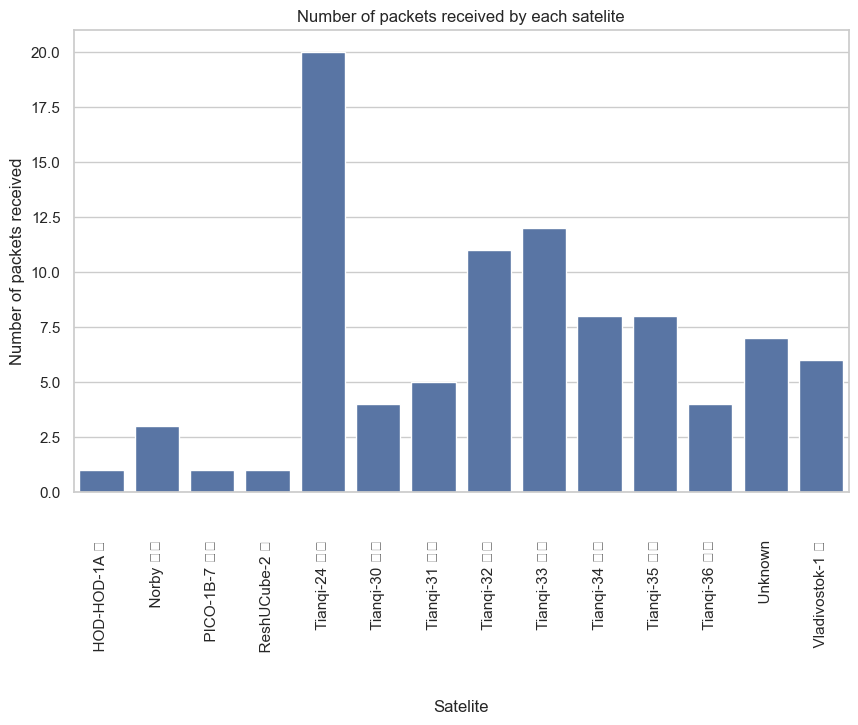
\includegraphics[width=0.8\textwidth]{../images/satelites.png}
    \caption{Data received from 15 satellites most prominent being Tianqi-24}
    \label{fig:received_data}
\end{figure}
Even though the LILYGO operated at 433MHz ideally the data varied from 400MHz to 460MHz and this was mostly characteristic of the quater wave ground plane antenna. However most data was close to the 400MHz mark as seen in the plot below.
\begin{figure}[H]
    \centering
    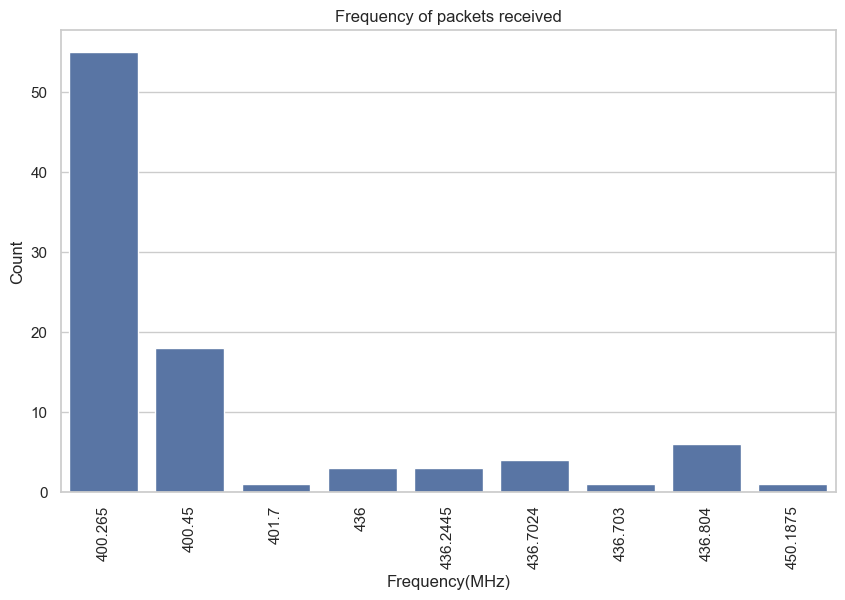
\includegraphics[width=0.8\textwidth]{../images/frequencies.png}
    \caption{Frequency of data received from the satellites}
    \label{fig:frequency_data}
\end{figure}

% 'Description for 📐 Elevation:'
% count    91.000000
% mean     25.450440
% std      17.576382
% min       0.510000
% 25%      11.365000
% 50%      21.840000
% 75%      32.845000
% max      65.950000
% Name: 📐 Elevation, dtype: float64
The Elevation angle of the satellites was also analyzed. The data showed that the average elevation angle was approximately 25.45 degrees, with a maximum elevation angle of 65.95 degrees. This indicates that the ground station had a good view of the sky, allowing for effective communication with the satellites.
\begin{figure}[H]
    \centering
    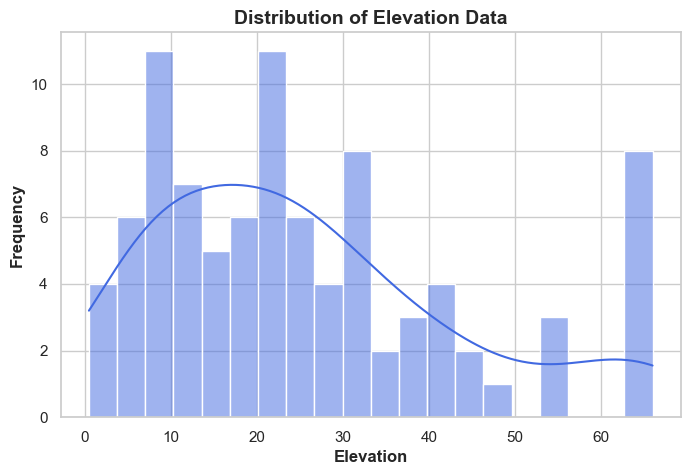
\includegraphics[width=0.8\textwidth]{../images/elevation.png}
    \caption{Elevation angle of the satellites}
    \label{fig:elevation_data}
\end{figure}

Most Data was received from 15:00 hours to 17:00 hours and from 20:00 hour to 22:00 hours. This is when the satellites were most visible in the sky, allowing for effective communication with the ground station. There existed satelite shortages where the satelites which were transmitting data were to far from the ground station and thus no data was received.

\begin{figure}[H]
    \centering
    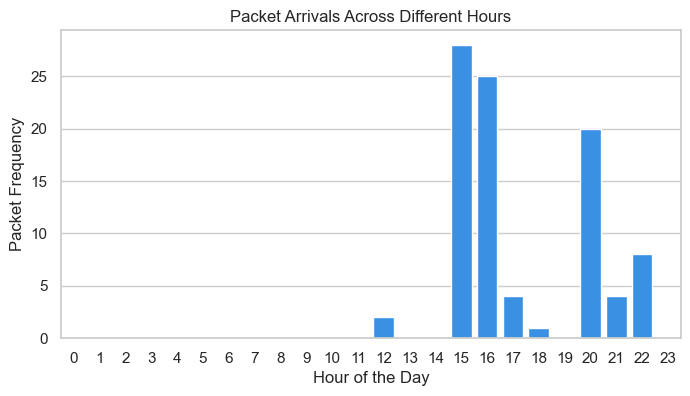
\includegraphics[width=0.8\textwidth]{../images/daytime.png}
    \caption{Time of data received from the satellites}
    \label{fig:time_data}
\end{figure}

The heatmap below shows the frequencies of data reception forr the different hours of the day for the days the satelite was deployed. It is clear most data was received between 3pm and 4pm. and then a period of scarcity follows.
\begin{figure}[H]
    \centering
    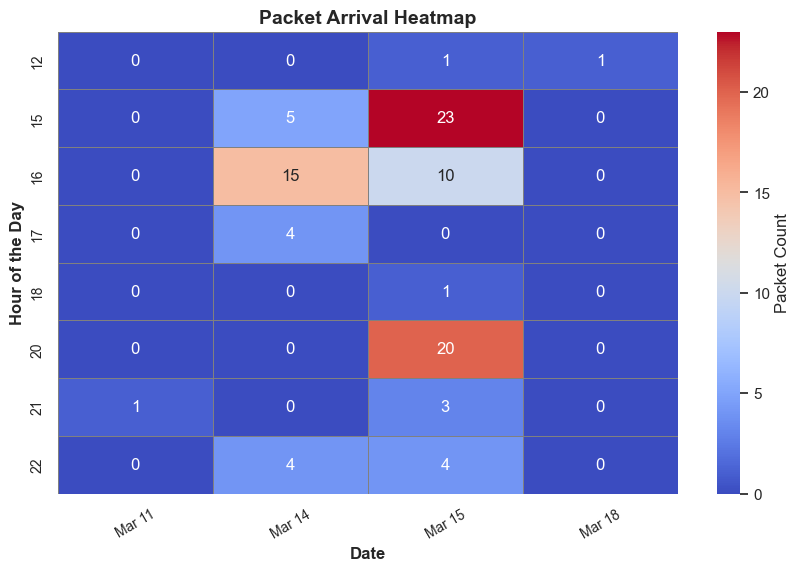
\includegraphics[width=0.8\textwidth]{../images/heatmap.png}
    \caption{Frequencies of data received for the different hours of the day}
    \label{fig:frequencies_data}
\end{figure}

% count      91.000000
% mean     1768.065934
% std       715.643375
% min       525.000000
% 25%      1171.000000
% 50%      1720.000000
% 75%      2337.500000
% max      3433.000000
% Name: 📏 Distance, dtype: float64
The average distance of satelite from station was 1768.07km with a maximum distance of 3433km. This is a good distance for the ground station to be able to receive data from the satellites. The distance was also analyzed in relation to the elevation angle of the satellites. The data showed that there was a negative correlation between the distance and elevation angle, indicating that as the elevation angle increased, the distance from the ground station decreased.

\begin{figure}[H]
    \centering
    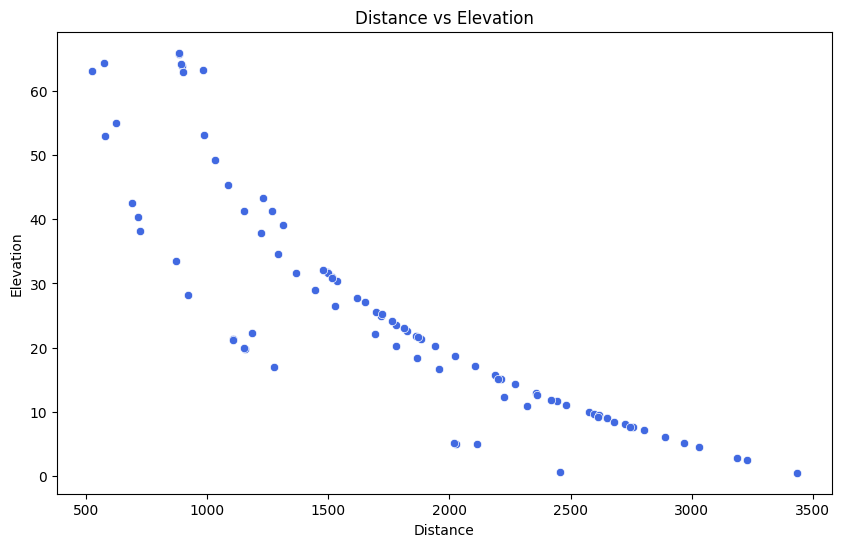
\includegraphics[width=0.8\textwidth]{../images/corr.png}
    \caption{Distance of the satellites vs Elevation from the ground station}
    \label{fig:distance_data}
\end{figure}

%  Conclusion and recomendations and challenges
\section{Conclusion}
The TinyGS project provides a cost-effective and versatile solution for building a LoRa satellite ground station. The installation and configuration process was straightforward, and the antenna design was effective in receiving data from satellites. The data analysis showed that the ground station performed well, with good reception of packets from multiple satellites.
The average elevation angle and distance of the satellites indicated that the ground station had a good view of the sky, allowing for effective communication. The data reception was highest during specific hours of the day, indicating that the ground station was able to effectively communicate with the satellites during these times.
The project was successful in demonstrating the feasibility of building a LoRa satellite ground station using the TinyGS project. The data analysis provided valuable insights into the performance of the ground station and highlighted areas for improvement.
Future work could focus on optimizing the antenna design for better performance and exploring additional features of the TinyGS project. The project also highlighted the importance of having a clear view of the sky for effective communication with satellites.
\section{Challenges}
The project faced several challenges, including:
\begin{itemize}
    \item Limited access to satellite data during certain times of the day.
    \item Issues with the antenna design, leading to poor reception of packets from satellites.
    \item Difficulty in analyzing the data received from the satellites as there wasn't an obviuos way to download the data.
    \item Limited knowledge and experience with radio engineering and satellite communication.
\end{itemize}
These challenges were addressed through collaboration with the TinyGS community and by leveraging online resources for troubleshooting and support. The project team also gained valuable experience in radio engineering and satellite communication, which will be beneficial for future projects.
\section{Recommendations}
The following recommendations were made based on the project experience:
\begin{itemize}
    \item Consider using a more advanced antenna design for better performance.
    \item Explore additional features of the TinyGS project for improved functionality.
    \item Collaborate with the TinyGS community for support and troubleshooting.
    \item Consider deploying an MQTT server so as to have our own data stream.
    \item Explore opportunities for collaboration with other ground stations for improved data sharing and analysis.
    \item Consider using more advanced hardware for better performance and reliability. Such as a better deployment site
\end{itemize}
\section{Acknowledgements}
The project team would like to thank the TinyGS community noticably Stefan for their support and resources, which were invaluable in the successful completion of this project. Special thanks to the developers of the TinyGS project for their hard work and dedication in creating a cost-effective and versatile solution for building LoRa satellite ground stations.
The project team would also like to thank the University of Makerere and in particular Dr Jonathan Sserugunda for providing the resources and support needed to complete this project.

\bibliographystyle{ieeetr}
\begin{thebibliography}{1}
    \bibitem{tinygs} TinyGS Project. Available at \url{https://tinygs.com}.
    \bibitem{tinygsinstaller} TinyGS Firmware Installer. Available at \url{http://installer.tinygs.com}.
    \bibitem{latlong} Latitude and Longitude Finder. Available at \url{http://latlong.net}.
    \bibitem{n1gyantenna} Simple Ground Plane Antennas. Available at \url{http://www.n1gy.com/simple-ground-plane-antennas.html}.
\end{thebibliography}

\end{document}
